%===============================================================================
\chapter{Modelo de comportamiento del subsistema: Gestión de tareas}
\label{cap:reqSist}

En este capítulo se describen los casos de uso referentes a la gestión, asiganción de responsables y asignación de dependencias de las tareas de un proyecto.

%---------------------------------------------------------

\begin{shaded}
		\textcolor{NavyBlue}{\Large\textbf{Elementos de un caso de uso}}
		\begin{itemize}
			\item \textbf{Resumen:} Descrpción textual del caso de uso
			\item \textbf{Actores:} Lista de los que  intervienen en el caso de uso.
			\item \textbf{Propósito:} Una breve descripción del objetivo que busca e actor al ejecutare el caso de uso.
			\item \textbf{Entradas:} Lista de los datos requeridos durante a ejecución del caso de uso.
			\item \textbf{Salidas:} Lista de los datos de salida que presetan al sistema durante la ejecuciń del caso de uso.
			\item \textbf{Precondiciones:} Descrpción de las operaciones o condiciones que se deben cumplir previamente para el caso de uso pueda ejecutarse correctamente.
			\item \textbf{Postcondiciones:} Lista de los cambios que ocurrirán en el sistema después de la ejecución del caso de uso y de las consecuencias del sistema.
			\item \textbf{Reglase de negocio:} Lista de las reglas que describen, limitan o controlan algún aspecto del negocio del caso de uso.
			\item \textbf{Errores:} Lista de los posibles errores que pueden surgir surante la ejecución del caso de uso.
			\item \textbf{Trayectoria:} Secuencia de los pasos que ejecutará el caso de uso
		\end{itemize}		
	\end{shaded}
\newpage

%-------------------------------------------------------------------------
%====================================================================================
\begin{UseCase}{CU20}{Configuración de tareas}{
		Permite al Lider de proyecto configurar las tareas que se realizaranen el proyecto, poder visuizaras en un diagrama de gantt y gestionar los avances atraves de un diagrama de representacion de avances por tareas.
	}
		\UCitem{Actor}{\hyperlink{LiderProyecto}{Lider de proyecto}}
		\UCitem{Propósito}{Permite al Lider de proyecto configurar las tareas que se realizaranen el proyecto, poder visuizaras en un diagrama de gantt y gestionar los avances atraves de un diagrama de representacion de avances por tareas.}
		\UCitem{Entradas}{Ninguna}
		\UCitem{Salidas}{Ninguna}
		\UCitem{Destino}{Pantalla de configuracion de tareas}
		\UCitem{Precondiciones}{Que el proyecto no este finalizado}
		\UCitem{Postcondiciones}{Ningunó}
		\UCitem{Errores}{Ningunó}
		\UCitem{Observaciones}{}
	\end{UseCase}
%--------------------------------------
	\begin{UCtrayectoria}{Principal}
		\UCpaso[\UCactor] Da click en el icono 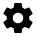
\includegraphics[height=10pt]{./images/iconos/ic_settings_black_18dp.png}
        \UCpaso [\UCsist] accede a la pantalla \hyperref[fig:IU20]{IU20 Configuración de tareas}.
        \UCpaso [\UCactor] puede gestionar la tareas atravez de la pestaña de 'Tareas' y se pueden gestinar atravez del boton,'Nueva tarea' y los iconos 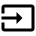
\includegraphics[height=10pt]{./images/iconos/ic_input_black_18dp.png},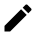
\includegraphics[height=10pt]{./images/iconos/ic_create_black_18dp.png},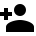
\includegraphics[height=10pt]{./images/iconos/ic_person_add_black_18dp.png},
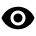
\includegraphics[height=10pt]{./images/iconos/ic_visibility_black_18dp.png},
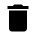
\includegraphics[height=10pt]{./images/iconos/ic_delete_black_18dp.png} \label{item:cu20Item1}       
        
	\end{UCtrayectoria}
%-------------------------------------------------
\subsection{Puntos de extensión del caso de uso}
\UCExtenssionPoint{El lider de proyecto desea relacionar las tareas presionando el icono 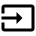
\includegraphics[height=10pt]{./images/iconos/ic_input_black_18dp.png}}{Continua en el paso \ref{item:cu20Item1} del \UCref{CU20}.}{\UCref{CU21}{ Relacionar Tareas}}

\UCExtenssionPoint{El lider de proyecto desea asignar colaboradores a la tarea presionando el icono 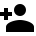
\includegraphics[height=10pt]{./images/iconos/ic_person_add_black_18dp.png}}{Continua en el paso \ref{item:cu20Item1} del \UCref{CU20}.}{\UCref{CU21}{ Relacionar Tareas}}

\UCExtenssionPoint{El lider de proyecto desea editar los datos de la tarea presionando el icono 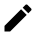
\includegraphics[height=10pt]{./images/iconos/ic_create_black_18dp.png}}{Continua en el paso \ref{item:cu20Item1} del \UCref{CU22}.}{\UCref{CU22}{ Editar Tarea}}

\UCExtenssionPoint{El lider de proyecto desea ver los datos generales de la tarea presionando el icono 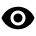
\includegraphics[height=10pt]{./images/iconos/ic_visibility_black_18dp.png}}{Continua en el paso \ref{item:cu20Item1} del \UCref{CU22}.}{\UCref{CU23}{ Visualizar Datos Tareas}}

\UCExtenssionPoint{El lider de proyecto desea eliminar la tarea presionando el icono 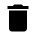
\includegraphics[height=10pt]{./images/iconos/ic_delete_black_18dp.png}}{Continua en el paso \ref{item:cu20Item1} del \UCref{CU22}.}{\UCref{CU24}{ Eliminar la tarea}}


%--------------------------------------		
		\begin{UCtrayectoriaA}{A}{ El actor no ingreso los datos requeridos}
			\UCpaso Muestra mensaje de falta de datos requeridos
			\UCpaso Continua en el paso \ref{item:CU19Item1} del \UCref{CU19}.
		\end{UCtrayectoriaA}
		
		
%-------------------------------------- TERMINA descripción del caso de uso.
%====================================================================================
\begin{UseCase}{CU21}{Relacionar Tareas}{
		Permite al Lider de proyecto relacionar las tareas configuradas para el proyeto, con el fin de ver que tareas dependen otras.
	}
		\UCitem{Actor}{\hyperlink{LiderProyecto}{Lider de proyecto}}
		\UCitem{Propósito}{Permite al Lider de proyecto relacionar las tareas configuradas para el proyeto, con el fin de ver que tareas dependen otras.}
		\UCitem{Entradas}{Tpo de relación: es el tipo de relacion que se tendra entre tareas, se selecciona de un catalogo de estas.}
		\UCitem{Salidas}{Relación entre una tarea y otra}
		\UCitem{Destino}{Pantalla de relación de tareas}
		\UCitem{Precondiciones}{Que existan tareas creadas para el proyecto}
		\UCitem{Postcondiciones}{Creación de la relación entre tareas}
		\UCitem{Errores}{\begin{itemize}
			\item El tipo de relacion no es posible: las fechas entre ellas difieren del tipo seleccionado.
			\item Campos obligatorios.	
		\end{itemize}}
		\UCitem{Observaciones}{}
	\end{UseCase}
%--------------------------------------
	\begin{UCtrayectoria}{Principal}
		\UCpaso[\UCactor] Da click en el icono 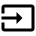
\includegraphics[height=10pt]{./images/iconos/ic_input_black_18dp.png}
        \UCpaso [\UCsist] accede a la pantalla \hyperref[fig:IU21]{IU21 Relacionar Tareas}.
        \UCpaso [\UCactor] puede agregar la relacion entre tareas a traves del icono 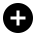
\includegraphics[height=10pt]{./images/iconos/ic_add_circle_black_18dp.png} y puede eliminar la relacion entre tareas presionando el icono 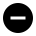
\includegraphics[height=10pt]{./images/iconos/ic_remove_circle_black_18dp.png} \label{item:cu21Item1}       
        
	\end{UCtrayectoria}
%-------------------------------------------------
\subsection{Puntos de extensión del caso de uso}
\UCExtenssionPoint{El lider de proyecto desea relacionar las tareas presionando el icono 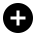
\includegraphics[height=10pt]{./images/iconos/ic_add_circle_black_18dp.png}}{Continua en el paso \ref{item:cu21Item1} del \UCref{CU21}.}{\UCref{CU25}{ Registrar relacion de tarea}}

\UCExtenssionPoint{El lider de proyecto desea eliminar la relacion entre tareas presionando el icono 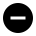
\includegraphics[height=10pt]{./images/iconos/ic_remove_circle_black_18dp.png}}{Continua en el paso \ref{item:cu21Item1} del \UCref{CU21}.}{\UCref{CU26}{ Remover relación de tarea}}
		
		
%-------------------------------------- TERMINA descripción del caso de uso.
%====================================================================================
\begin{UseCase}{CU22}{Editar tareas}{
		Permite al Lider de proyecto modificar los paramtros de la tarea seleccionad para editar.
	}
		\UCitem{Actor}{\hyperlink{LiderProyecto}{Lider de proyecto}}
		\UCitem{Propósito}{Permite al Lider de proyecto modificar los paramtros de la tarea seleccionad para editar.}
		\UCitem{Entradas}{\begin{itemize}
			\item Nombre: se ingresa desde el teclado.
			\item Tipo de duración: se presiona alguno de los radios.
			\item Fecha de inicio: se ingresa desde teclado.
			\item Fecha de término: se ingresa desde teclado.
			\item Duracion en dias: se ingresa desde teclado
			\item Descripción: se ingresa desde teclado.
		\end{itemize}}
		\UCitem{Salidas}{Tarea: tarea con parametros modificados}
		\UCitem{Destino}{Pantalla de gestión de tareas}
		\UCitem{Precondiciones}{Que la tarea no este finalizada}
		\UCitem{Postcondiciones}{Tarea modificada}
		\UCitem{Errores}{\begin{itemize}
			\item La fecha de inicio no puede ser mayor a la fecha de término.
			\item Campos obligatorios.	
		\end{itemize}}
		\UCitem{Observaciones}{}
	\end{UseCase}
%--------------------------------------
	\begin{UCtrayectoria}{Principal}
		\UCpaso[\UCactor] Da click en el icono 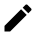
\includegraphics[height=10pt]{./images/iconos/ic_create_black_18dp.png}
        \UCpaso [\UCsist] abre el cuadro de dialogo \hyperref[fig:IU22]{IU22 Editar tarea}.
        \UCpaso [\UCactor] puede agregar la relacion entre tareas a traves del icono 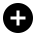
\includegraphics[height=10pt]{./images/iconos/ic_add_circle_black_18dp.png} y puede eliminar la relacion entre tareas presionando el icono 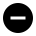
\includegraphics[height=10pt]{./images/iconos/ic_remove_circle_black_18dp.png} \label{item:cu21Item1}       
        
	\end{UCtrayectoria}
%-------------------------------------------------
\subsection{Puntos de extensión del caso de uso}
\UCExtenssionPoint{El lider de proyecto desea relacionar las tareas presionando el icono 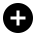
\includegraphics[height=10pt]{./images/iconos/ic_add_circle_black_18dp.png}}{Continua en el paso \ref{item:cu21Item1} del \UCref{CU21}.}{\UCref{CU25}{ Registrar relacion de tarea}}

\UCExtenssionPoint{El lider de proyecto desea eliminar la relacion entre tareas presionando el icono 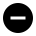
\includegraphics[height=10pt]{./images/iconos/ic_remove_circle_black_18dp.png}}{Continua en el paso \ref{item:cu21Item1} del \UCref{CU21}.}{\UCref{CU26}{ Remover relación de tarea}}
		
		
%-------------------------------------- TERMINA descripción del caso de uso.
%====================================================================================
\begin{UseCase}{CU23}{Visualizar datos de la tarea}{
		Permite al Lider de proyecto visualizar los datos generales de la tarea.
	}
		\UCitem{Actor}{\hyperlink{LiderProyecto}{Lider de proyecto}}
		\UCitem{Propósito}{Permite al Lider de proyecto visualizar los datos generales de la tarea.}
		\UCitem{Entradas}{Ninguna}
		\UCitem{Salidas}{Nnguna}
		\UCitem{Destino}{Pantalla de gestión de tareas}
		\UCitem{Precondiciones}{Ninguna}
		\UCitem{Postcondiciones}{Ninguna}
		\UCitem{Errores}{}
		\UCitem{Observaciones}{}
	\end{UseCase}
%--------------------------------------
	\begin{UCtrayectoria}{Principal}
		\UCpaso[\UCactor] Da click en el icono 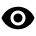
\includegraphics[height=10pt]{./images/iconos/ic_visibility_black_18dp.png}
        \UCpaso [\UCsist] accede a la pantalla \hyperref[fig:IU23]{IU23 Visualizar datos de la tarea}. \Trayref{A}
	\end{UCtrayectoria}
%-------------------------------------------------
\begin{UCtrayectoriaA}{A}{ El actor presiona el boton 'regresar'}
			\UCpaso [\UCsist] accede a la pantalla \hyperref[fig:IU20]{IU20 Configuración de tareas}.
		\end{UCtrayectoriaA}		
		
%-------------------------------------- TERMINA descripción del caso de uso.
%====================================================================================
\begin{UseCase}{CU24}{Eliminar tarea}{
		Permite al Lider de proyecto eliminar la tarea que seleccione.
	}
		\UCitem{Actor}{\hyperlink{LiderProyecto}{Lider de proyecto}}
		\UCitem{Propósito}{Permite al Lider de proyecto eliminar la tarea que seleccione.}
		\UCitem{Entradas}{Ninguna}
		\UCitem{Salidas}{Nnguna}
		\UCitem{Destino}{Pantalla de gestión de tareas}
		\UCitem{Precondiciones}{no se encuntre finalizada a tarea seleccionada}
		\UCitem{Postcondiciones}{tarea eliminada}
		\UCitem{Errores}{}
		\UCitem{Observaciones}{}
	\end{UseCase}
%--------------------------------------
	\begin{UCtrayectoria}{Principal}
		\UCpaso[\UCactor] Da click en el icono 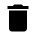
\includegraphics[height=10pt]{./images/iconos/ic_delete_black_18dp.png}
        \UCpaso [\UCsist] abre el cuadro de dialogo preguntando '¿Desea elimnar la tarea seleccionada'. \Trayref{A} \label{item:CU24Item1}
	\end{UCtrayectoria}
%-------------------------------------------------
\begin{UCtrayectoriaA}{A}{ La tarea ya esta finalizada}
			\UCpaso [\UCsist] Muestra el mensaje 'No se puede eliminar una materia finaizada'.
			\UCpaso [\UCsist] Continua en el paso \ref{item:CU24Item1} del \UCref{CU24}.
		\end{UCtrayectoriaA}		
		
%-------------------------------------- TERMINA descripción del caso de uso.
%====================================================================================
\begin{UseCase}{CU25}{Registrar relacion de tarea}{
		Permite al Lider de proyecto de una tarea relacionarla a otra.
	}
		\UCitem{Actor}{\hyperlink{LiderProyecto}{Lider de proyecto}}
		\UCitem{Propósito}{Permite al Lider de proyecto de una tarea relacionarla a otra.}
		\UCitem{Entradas}{Tipo de relación: selecconada desde select con el catalogo.}
		\UCitem{Salidas}{Tarea: tarea relacionada a la tarea actual.}
		\UCitem{Destino}{Pantalla de relacion de tareas}
		\UCitem{Precondiciones}{se allá selecconado un tipo de relacion para el registro de la relacion con la tarea actual.}
		\UCitem{Postcondiciones}{tarea relacionada con la actual}
		\UCitem{Errores}{\begin{itemize}
			\item Campos obligatorios.
			\item El tipo de relacion no esta permitida por las fechas registradas para las tareas.
		\end{itemize}}
		\UCitem{Observaciones}{}
	\end{UseCase}
%--------------------------------------
	\begin{UCtrayectoria}{Principal}
		\UCpaso [\UCactor] selecciona un tipo de relación para la tarea que seleccione.
		\UCpaso[\UCactor] Da click en el icono 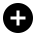
\includegraphics[height=10pt]{./images/iconos/ic_add_circle_black_18dp.png}. \label{item:CU25Item1}
        \UCpaso [\UCsist] verifica que el select tenga una opcion seleccionada. \Trayref{A}
        \UCpaso [\UCsist] verifica que las fechas de la tarea actual y la tarea seleccionada para relacionar esten permitidas para el tipo de relación seleccionada. \Trayref{B}
	\end{UCtrayectoria}
%-------------------------------------------------
\begin{UCtrayectoriaA}{A}{No se selecciono una opción valida}
			\UCpaso [\UCsist] Muestra el mensaje 'Campos obligatorios'.
			\UCpaso [\UCsist] Continua en el paso \ref{item:CU25Item1} del \UCref{CU24}.
		\end{UCtrayectoriaA}
		
		\begin{UCtrayectoriaA}{B}{El tipo de relación no es posible por las fechas de la tareas}
			\UCpaso [\UCsist] Muestra el mensaje 'El tipo de relacion no esta permitida por las fechas registradas para las tareas.'.
			\UCpaso [\UCsist] Continua en el paso \ref{item:CU25Item1} del \UCref{CU24}.
		\end{UCtrayectoriaA}		
		
%-------------------------------------- TERMINA descripción del caso de uso.
%====================================================================================
\begin{UseCase}{CU26}{Remover relación de tarea}{
		Permite al Lider de proyecto remover la reación de tareas.
	}
		\UCitem{Actor}{\hyperlink{LiderProyecto}{Lider de proyecto}}
		\UCitem{Propósito}{permitir al lider de proyecto remover la reación de tareas.}
		\UCitem{Entradas}{Ninguna}
		\UCitem{Salidas}{relacion entre tareas removida.}
		\UCitem{Destino}{Pantalla de relacion de tareas.}
		\UCitem{Precondiciones}{tener relaciones registradas.}
		\UCitem{Postcondiciones}{relacion removida.}
		\UCitem{Errores}{Ninguna}
		\UCitem{Observaciones}{}
	\end{UseCase}
%--------------------------------------
	\begin{UCtrayectoria}{Principal}
		\UCpaso[\UCactor] Da click en el icono 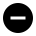
\includegraphics[height=10pt]{./images/iconos/ic_remove_circle_black_18dp.png}.
        \UCpaso [\UCsist] removera la relación seleccionada.
	\end{UCtrayectoria}
		
%-------------------------------------- TERMINA descripción del caso de uso.
%====================================================================================
\begin{UseCase}{CU27}{Ver diagrama de gantt}{
		Permite al Lider de proyecto ver el diagrama de gantt conteniente de las tareas de proyecto.
	}
		\UCitem{Actor}{\hyperlink{LiderProyecto}{Lider de proyecto}}
		\UCitem{Propósito}{permitir al Lider de proyecto ver el diagrama de gantt conteniente de las tareas de proyecto.}
		\UCitem{Entradas}{Ninguna}
		\UCitem{Salidas}{Ninguna}
		\UCitem{Destino}{Pantalla de configuración de tareas.}
		\UCitem{Precondiciones}{tener tareas registradas.}
		\UCitem{Postcondiciones}{generación del diagrama de gantt}
		\UCitem{Errores}{Ninguna}
		\UCitem{Observaciones}{}
	\end{UseCase}
%--------------------------------------
	\begin{UCtrayectoria}{Principal}
		\UCpaso[\UCactor] Da click en la pestaña 'Gantt' de la pantalla \hyperref[fig:IU27]{IU27 Ver diagrama de gantt}.
        \UCpaso [\UCsist] buscara la lista de tareas registradas para el proyecto.
        \UCpaso [\UCsist]  generara el diagrama de gantt con todas las tareas registradas, así como sus relaciones.
	\end{UCtrayectoria}
		
%-------------------------------------- TERMINA descripción del caso de uso.
%====================================================================================
\begin{UseCase}{CU28}{Ver estadisticas de avances de las tareas}{
		Permite al Lider de proyecto ver las estadistias de los avances de las tareas registradas en el proyecto.
	}
		\UCitem{Actor}{\hyperlink{LiderProyecto}{Lider de proyecto}}
		\UCitem{Propósito}{permitir al Lider de proyecto ver las estadistias de los avances de las tareas registradas en el proyecto.}
		\UCitem{Entradas}{Ninguna}
		\UCitem{Salidas}{Ninguna}
		\UCitem{Destino}{Pantalla de configuración de tareas.}
		\UCitem{Precondiciones}{tener tareas registradas.}
		\UCitem{Postcondiciones}{generación del diagrama de gantt}
		\UCitem{Errores}{Ninguna}
		\UCitem{Observaciones}{}
	\end{UseCase}
%--------------------------------------
	\begin{UCtrayectoria}{Principal}
		\UCpaso[\UCactor] Da click en la pestaña 'Estadisticas' de la pantalla \hyperref[fig:IU28]{IU20 Configuración de tareas}.
        \UCpaso [\UCsist] buscara la lista de tareas registradas para el proyecto.
        \UCpaso [\UCsist]  generara los diagramas de reportes de avances de tareas.
	\end{UCtrayectoria}
		
%-------------------------------------- TERMINA descripción del caso de uso.
%====================================================================================
\begin{UseCase}{CU29}{Mis tareas}{
		Permite al Lider de proyecto y al colaborador, ver la tareas que tinen asignadas en el proyecto que estan participando.
	}
		\UCitem{Actor}{\hyperlink{LiderProyecto}{Lider de proyecto}}
		\UCitem{Propósito}{permitir al Lider de proyecto y al colaborador, ver la tareas que tinen asignadas en el proyecto que estan participando.}
		\UCitem{Entradas}{Ninguna}
		\UCitem{Salidas}{Ninguna}
		\UCitem{Destino}{Pantalla de Mis tareas.}
		\UCitem{Precondiciones}{tener tareas asignadas.}
		\UCitem{Postcondiciones}{Ninguna}
		\UCitem{Errores}{Ninguna}
		\UCitem{Observaciones}{}
	\end{UseCase}
%--------------------------------------
	\begin{UCtrayectoria}{Principal}
		\UCpaso[\UCactor] Da click en el icono 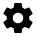
\includegraphics[height=10pt]{./images/iconos/ic_settings_black_18dp.png}.
		\UCpaso[\UCsist] accede a la pantalla \hyperref[fig:IU29]{IU29 Mis tareas}.
        \UCpaso [\UCsist] buscara la lista de tareas en las que el lider o colaborador se encuentren asignado para el proyecto. \label{item:cu29Item1}
	\end{UCtrayectoria}

%---------------------------------------
\subsection{Puntos de extensión del caso de uso}
\UCExtenssionPoint{El lider de proyecto o el colaborador desea reporter sus avances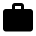
\includegraphics[height=10pt]{./images/iconos/ic_work_black_18dp.png}}{Continua en el paso \ref{item:cu29Item1} del \UCref{CU29}.}{\UCref{CU30}{ Avances de tareas}}
%-------------------------------------- TERMINA descripción del caso de uso.
%====================================================================================
\begin{UseCase}{CU30}{Avances de tareas}{
		Permite al Lider de proyecto y al colaborador, ver y reportar los avances que tenga en las tareas.
	}
		\UCitem{Actor}{\hyperlink{LiderProyecto}{Lider de proyecto}, \hyperlink{Colaborador}{Colaborador}}
		\UCitem{Propósito}{permitir al Lider de proyecto y al colaborador, ver y reportar los avances que tenga en las tareas.}
		\UCitem{Entradas}{Ninguna}
		\UCitem{Salidas}{Ninguna}
		\UCitem{Destino}{Pantalla de Mis tareas.}
		\UCitem{Precondiciones}{la tarea no este finalizada.}
		\UCitem{Postcondiciones}{Ninguna}
		\UCitem{Errores}{Ninguna}
		\UCitem{Observaciones}{}
	\end{UseCase}
%--------------------------------------
	\begin{UCtrayectoria}{Principal}
		\UCpaso[\UCactor] Da click en el icono 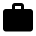
\includegraphics[height=10pt]{./images/iconos/ic_work_black_18dp.png}.
		\UCpaso[\UCsist] accede a la pantalla \hyperref[fig:IU30]{IU30 Avances de tareas}.
        \UCpaso [\UCsist] verificara que la tarea no este finalizada \label{item:cu30Item1}
        \UCpaso [\UCactor] puede reportar sus tareas a traves de los iconos 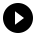
\includegraphics[height=10pt]{./images/iconos/ic_play_circle_filled_black_18dp.png},
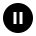
\includegraphics[height=10pt]{./images/iconos/ic_pause_circle_filled_black_18dp.png},
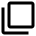
\includegraphics[height=10pt]{./images/iconos/ic_filter_none_black_18dp.png}.\label{item:cu30Item2}
	\end{UCtrayectoria}

%---------------------------------------
	\begin{UCtrayectoriaA}{A}{ La tarea esta finalizada}
			\UCpaso [\UCpaso] Muestra mensaje 'La tarea ha finalizado no se puede reportar avances'
			\UCpaso Continua en el paso \ref{item:CU30Item1} del \UCref{CU30}.
		\end{UCtrayectoriaA}

%---------------------------------------
\subsection{Puntos de extensión del caso de uso}
\UCExtenssionPoint{El lider de proyecto o el colaborador desea reporter sus avances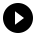
\includegraphics[height=10pt]{./images/iconos/ic_play_circle_filled_black_18dp.png}}{Continua en el paso \ref{item:cu30Item2} del \UCref{CU30}.}{\UCref{CU10}{ Iniciar Tarea}}

\UCExtenssionPoint{El lider de proyecto o el colaborador desea pausar la tarea en curso 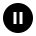
\includegraphics[height=10pt]{./images/iconos/ic_pause_circle_filled_black_18dp}}{Continua en el paso \ref{item:cu30Item2} del \UCref{CU30}.}{\UCref{CU11}{ Pausar Tarea}}

\UCExtenssionPoint{El lider de proyecto o el colaborador desea ver los avances de su commit 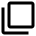
\includegraphics[height=10pt]{./images/iconos/ic_filter_none_black_18dp.png}}{Continua en el paso \ref{item:cu30Item2} del \UCref{CU30}.}{\UCref{CU31}{ Ver avances commit}}
%-------------------------------------- TERMINA descripción del caso de uso.
%====================================================================================
\begin{UseCase}{CU31}{Ver avances commit}{
		Permite al Lider de proyecto y al colaborador, ver los detalles del avance del commit.
	}
		\UCitem{Actor}{\hyperlink{LiderProyecto}{Lider de proyecto}, \hyperlink{Colaborador}{Colaborador}}
		\UCitem{Propósito}{permitir al Lider de proyecto y al colaborador, ver los detalles del avance del commit.}
		\UCitem{Entradas}{Ninguna}
		\UCitem{Salidas}{Ninguna}
		\UCitem{Destino}{Avances de commit}
		\UCitem{Precondiciones}{Ninguna}
		\UCitem{Postcondiciones}{Ninguna}
		\UCitem{Errores}{Ninguna}
		\UCitem{Observaciones}{}
	\end{UseCase}
%--------------------------------------
	\begin{UCtrayectoria}{Principal}
		\UCpaso[\UCactor] Da click en el icono 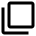
\includegraphics[height=10pt]{./images/iconos/ic_filter_none_black_18dp.png}.
		\UCpaso[\UCsist] accede a la pantalla \hyperref[fig:IU31]{IU31 Ver avances commit}. \label{item:cu30Item1}
	\end{UCtrayectoria}

%---------------------------------------
	\begin{UCtrayectoriaA}{A}{ El actor presiona el botón 'regresar'}
			\UCpaso regresa a la pantalla la pantalla \hyperref[fig:IU30]{IU30 Avance de tareas}.
		\end{UCtrayectoriaA}

%-------------------------------------- TERMINA descripción del caso de uso.
% \IUref{IUAdmPS}{Administrar Planta de Selección}
% \IUref{IUModPS}{Modificar Planta de Selección}
% \IUref{IUEliPS}{Eliminar Planta de Selección}

% 


% Copie este bloque por cada caso de uso:
%-------------------------------------- COMIENZA descripción del caso de uso.

%\begin{UseCase}[archivo de imágen]{UCX}{Nombre del Caso de uso}{
%--------------------------------------
	\begin{UseCase}{CU04}{Crear tarea}{
		Permite a un usuario la creación de una tarea en un proyecto ya creado.
	}
		\UCitem{Actor}{\hyperlink{Líder de proyecto}{Líder de proyecto}}
		\UCitem{Propósito}{Definir una tarea que pertenece a un proyecto.}
		\UCitem{Entradas}{\begin{itemize}
		\item Proyecto: Lo obtiene el sistema
\item Fecha de inicio: Se selecciona de un calendario
\item Fecha de térmico: Se selecciona de un calendario
\item Descripción: Se ingresa desde el teclado


		\end{itemize}
.}
		\UCitem{Salidas}{Tarea asignada: Lo genera el sistema.}
		\UCitem{Destino}{Pantalla de tareas del proyectos}
		\UCitem{Precondiciones}{Haber iniciado sesión y tener un proyecto creado
}
		\UCitem{Postcondiciones}{La tarea queda registrada en el sistema }
		\UCitem{Errores}{La fecha está fuera del rango del proyecto, la fecha de término es anterior a la fecha de inicio
}
		\UCitem{Observaciones}{}
	\end{UseCase}
%--------------------------------------
	\begin{UCtrayectoria}{Principal}
		\UCpaso[\UCactor] Da click en el menú de proyectos.
		\UCpaso[\UCactor] Da click en el ícono de tareas en la lista de proyectos.
        \UCpaso Muestra la pantalla de listado de tareas. 
       \UCpaso[\UCactor] Da click en el botón de crear tarea. 
       \UCpaso  Muestra la pantalla de crear tarea. \label{tarea}
      \UCpaso[\UCactor]  Ingresa el nombre, fecha de inicio, fecha de término y descripción.   \Trayref{A}
      \UCpaso[\UCactor]  Verifica que la fecha de inicio sea anterior a la fecha de fin.  \Trayref{B}
      \UCpaso[\UCactor]  Verifica que las fechas se encuentran dentro del rango del proyecto.    \Trayref{C}
       \UCpaso  Muestra la pantalla del listado de tareas.
	\end{UCtrayectoria}

%--------------------------------------		
		\begin{UCtrayectoriaA}{A}{ El actor no ingreso los datos requeridos}
			\UCpaso Muestra mensaje de falta de datos requeridos
			\UCpaso Continua en el paso \ref{tarea} del \UCref{CU04}.
		\end{UCtrayectoriaA}
%--------------------------------------		
		\begin{UCtrayectoriaA}{B}{ El actor ingresó una fecha de inicio inválida}
			\UCpaso Muestra mensaje de que las fechas no son válidas.
			\UCpaso Continua en el paso \ref{tarea} del \UCref{CU04}.
		\end{UCtrayectoriaA}
%--------------------------------------		
		\begin{UCtrayectoriaA}{C}{ El actor ingresó una fecha fuera del rango. }
			\UCpaso Muestra mensaje de que las fechas no son válidas.
			\UCpaso Continua en el paso \ref{tarea} del \UCref{CU04}.
		\end{UCtrayectoriaA}
		
		
%-------------------------------------- TERMINA descripción del caso de uso.
% \IUref{IUAdmPS}{Administrar Planta de Selección}
% \IUref{IUModPS}{Modificar Planta de Selección}
% \IUref{IUEliPS}{Eliminar Planta de Selección}

% 


% Copie este bloque por cada caso de uso:
%-------------------------------------- COMIENZA descripción del caso de uso.

%\begin{UseCase}[archivo de imágen]{UCX}{Nombre del Caso de uso}{
%--------------------------------------
	\begin{UseCase}{CU07}{Asignar tarea}{
		Permite a un usuario la asignación del responsable de una tarea.
	}
		\UCitem{Actor}{\hyperlink{Líder de proyecto.}{Líder de proyecto.}}
		\UCitem{Propósito}{Definir el responsable de una tarea.}
		\UCitem{Entradas}{\begin{itemize}
		\item Proyecto: Lo obtiene el sistema
		\item Tarea: Lo obtiene el sistema
		\item Colaborador: Se selecciona de una lista

		\end{itemize}
.}
		\UCitem{Salidas}{Tarea asignada: Lo genera el sistema  
}
		\UCitem{Destino}{Pantalla de tareas del proyecto.}
		\UCitem{Precondiciones}{Haber iniciado sesión, tener un proyecto creado, tener una tarea creada.
}
		\UCitem{Postcondiciones}{La tarea queda asignada a un colaborador en el sistema 
 }
		\UCitem{Errores}{}
		\UCitem{Observaciones}{}
	\end{UseCase}
%--------------------------------------
	\begin{UCtrayectoria}{Principal}
		\UCpaso[\UCactor]Da click en el menú de proyectos.
       \UCpaso [\UCactor]Da click en el ícono de tareas en la lista de proyectos.
      \UCpaso  Muestra la pantalla de listado de tareas. 
      \UCpaso [\UCactor]Da click en el ícono de asignar tarea. 
      \UCpaso Muestra la pantalla de asignar tarea. \label{asignar}
      \UCpaso[\UCactor] Selecciona un colaborador de una lista.   \Trayref{A} \Trayref{B} 
       \UCpaso   Muestra la pantalla del listado de tareas.
	\end{UCtrayectoria}

%--------------------------------------		
		\begin{UCtrayectoriaA}{A}{ El actor no selecciono ningún colaborador}
			\UCpaso Muestra mensaje de que no se ha seleccionado ningún colaborador.
			\UCpaso Continua en el paso \ref{asignar} del \UCref{CU07}.
		\end{UCtrayectoriaA}
        
        
%--------------------------------------		
		\begin{UCtrayectoriaA}{B}{El actor presiona el botón de cancelar.}
			\UCpaso Muestra la pantalla de listado de tareas.
		\end{UCtrayectoriaA}
		
		
%-------------------------------------- TERMINA descripción del caso de uso.
% \IUref{IUAdmPS}{Administrar Planta de Selección}
% \IUref{IUModPS}{Modificar Planta de Selección}
% \IUref{IUEliPS}{Eliminar Planta de Selección}

% 


% Copie este bloque por cada caso de uso:
%-------------------------------------- COMIENZA descripción del caso de uso.

%\begin{UseCase}[archivo de imágen]{UCX}{Nombre del Caso de uso}{
%--------------------------------------
	\begin{UseCase}{CU10}{Iniciar tarea}{
		Permite a un colaborador iniciar el reporte del tiempo invertido para resolver sobre una tarea asignada.
	}
		\UCitem{Actor}{\hyperlink{Colaborador.}{Colaborador.}}
		\UCitem{Propósito}{Reportar el tiempo invertido en una tara especifica.}
		\UCitem{Entradas}{\begin{itemize}
		\item Usuario: lo obtiene el sistema
		\item Proyecto: lo obtiene el sistema
		\item Tarea asignada: lo obtiene el sistema
		\end{itemize}
.}
		\UCitem{Salidas}{Tarea iniciada: Lo genera el sistema  
}
		\UCitem{Destino}{Tareas.}
		\UCitem{Precondiciones}{Tener una cuenta creada, tener una sesión iniciada, estar participando como colaborador en un proyecto y tener una tarea asignada.
}
		\UCitem{Postcondiciones}{La tarea pasa a estado de iniciada
 }
		\UCitem{Errores}{}
		\UCitem{Observaciones}{}
	\end{UseCase}
%--------------------------------------
	\begin{UCtrayectoria}{Principal}
      \UCpaso  Muestra la pantalla principal.
		\UCpaso[\UCactor]Da click en iniciar tarea en el icono 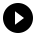
\includegraphics[height=10pt]{./images/iconos/ic_play_circle_filled_black_18dp.png}.
      \UCpaso  Hace un nuevo registro sobre la hora de inicio de la tarea.
	\end{UCtrayectoria}
		
%-------------------------------------- TERMINA descripción del caso de uso.
% \IUref{IUAdmPS}{Administrar Planta de Selección}
% \IUref{IUModPS}{Modificar Planta de Selección}
% \IUref{IUEliPS}{Eliminar Planta de Selección}

% 


% Copie este bloque por cada caso de uso:
%-------------------------------------- COMIENZA descripción del caso de uso.

%\begin{UseCase}[archivo de imágen]{UCX}{Nombre del Caso de uso}{
%--------------------------------------
	\begin{UseCase}{CU11}{Pausar tarea}{
		Permite a un colaborador detener el reporte del tiempo invertido para resolver una tarea asignada.
	}
		\UCitem{Actor}{\hyperlink{Colaborador.}{Colaborador.}}
		\UCitem{Propósito}{Reportar cuando el colaborador para de trabajar en una tara especifica.}
		\UCitem{Entradas}{\begin{itemize}
		\item Usuario: lo obtiene el sistema
		\item Proyecto: lo obtiene el sistema
		\item Tarea iniciada: lo obtiene el sistema
		\end{itemize}
.}
		\UCitem{Salidas}{Tarea pausada: Lo genera el sistema  
}
		\UCitem{Destino}{Tareas.}
		\UCitem{Precondiciones}{Tener una cuenta creada, tener una sesión iniciada, estar participando como colaborador en un proyecto, tener una tarea asignada y tener una tarea iniciada.
}
		\UCitem{Postcondiciones}{La tarea pasa a estado de pausada
 }
		\UCitem{Errores}{}
		\UCitem{Observaciones}{}
	\end{UseCase}
%--------------------------------------
	\begin{UCtrayectoria}{Principal}
      \UCpaso  Muestra la pantalla principal.
		\UCpaso[\UCactor]Da click en pausar tarea 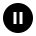
\includegraphics[height=10pt]{./images/iconos/ic_pause_circle_filled_black_18dp.png}.
      \UCpaso  Hace un nuevo registro sobre la hora en que se pauso la tarea.
	\end{UCtrayectoria}
		
%-------------------------------------- TERMINA descripción del caso de uso.
% \IUref{IUAdmPS}{Administrar Planta de Selección}
% \IUref{IUModPS}{Modificar Planta de Selección}
% \IUref{IUEliPS}{Eliminar Planta de Selección}

% 


% Copie este bloque por cada caso de uso:
%-------------------------------------- COMIENZA descripción del caso de uso.

%\begin{UseCase}[archivo de imágen]{UCX}{Nombre del Caso de uso}{
%--------------------------------------
	\begin{UseCase}{CU14}{Ver tareas}{
		Permite al líder de proyecto ver las tareas que ha creado en sus proyectos.
	}
		\UCitem{Actor}{\hyperlink{Líder de Proyecto.}{Líder de Proyecto.}}
		\UCitem{Propósito}{Controlar las tareas de mis proyectos.}
		\UCitem{Entradas}{\begin{itemize}
		\item Usuario: lo obtiene el sistema
		\item Proyecto: lo obtiene el sistema
		\item Tareas: lo obtiene el sistema
		\end{itemize}
.}
		\UCitem{Salidas}{Tareas: lo genera el sistema  
}
		\UCitem{Destino}{Tareas.}
		\UCitem{Precondiciones}{Tener una cuenta creada, tener una sesión iniciada, estar participando como líder en el proyecto. 
}
		\UCitem{Postcondiciones}{
 }
		\UCitem{Errores}{}
		\UCitem{Observaciones}{}
	\end{UseCase}
%--------------------------------------
	\begin{UCtrayectoria}{Principal}
      \UCpaso  Muestra la pantalla principal.
		\UCpaso[\UCactor]Da click en el menú de mis proyectos.
      \UCpaso  Muestra mis proyectos.
		\UCpaso[\UCactor]Da click en el ícono de configuración del proyecto.
      \UCpaso  Muestra la pantalla de tareas.
	\end{UCtrayectoria}

		
%-------------------------------------- TERMINA descripción del caso de uso.